\documentclass[12pt,a4paper]{article}
\usepackage[top=25.4mm, bottom=25.4mm, left=19.1mm, right=19.1mm]{geometry}

\usepackage[latin2]{inputenc}
\usepackage{graphicx}
\graphicspath{ {./images/} }
\usepackage{ulem}
\usepackage{amsmath}
\usepackage[document]{ragged2e}

\setlength{\parindent}{4em}
\setlength{\parskip}{1em}
\usepackage{hyperref}

\usepackage{fancyhdr}
\pagestyle{fancy}
\fancyhf{}
\fancyhead[LO]{\textbf{\small IoT and Smart Analytics}\\
\text{\small A Program by IIITH and TalentSprint}}

\usepackage{xcolor}
\usepackage{lipsum}

\rhead{\begin{picture}(0,0) \put(-250,-2){
\includegraphics[width=9cm]{EXP_08_Images/ts-iisc-logo-pr.png}} \end{picture}}
\cfoot{\thepage}


\begin{document}

\begin{center}

\textbf{\large \\EXPERIMENT 10 }\\[6pt]
\text{Non-Inverting Amplifier using LM358}
\end{center}

\textbf{\large LEARNING OBJECTIVES:}\\[3pt]
At the end of this experiment, participants will be able to:\vspace{-6mm}\begin{enumerate}
 \setlength\itemsep{-0.3em}
\item Understand LM358 application \\
\item Use LM358 to make a non-inverting amplifier of gain 10 \\

\end{enumerate}
\textbf{\large APPARATUS REQUIRED:}\\
\vspace{-3mm}
\begin{enumerate}
 \setlength\itemsep{-0.3em}
\item LM358 op-amp -1pcs \\
\item Potentiometer-1pcs\\
\item Power Adapter-1pcs\\
\item DC-DC Voltage Converter\\
\item Resistor 1k$\Omega$, 10k$\Omega$ - each 1pcs\\
\item Breadboard-1pcs\\
\item Jumper wires\\

\end{enumerate}

\begin{justify}
\textbf{\large THEORY}\\[3pt]
\textbf{Non-Inverting Amplifier:  } A non-inverting amplifier is an amplifier in which the circuit gives an amplified output signal where this output signal of the non-inverting op-amp is in-phase with the applied input signal. The input is applied to the non-inverting terminal for obtaining a non-inverted output. So the input signal does not change its polarity when it gets an amplified output at the output terminal.\\
Let us understand this by op-amp circuit with a feedback loop as shown below:
\par

\begin{center} 
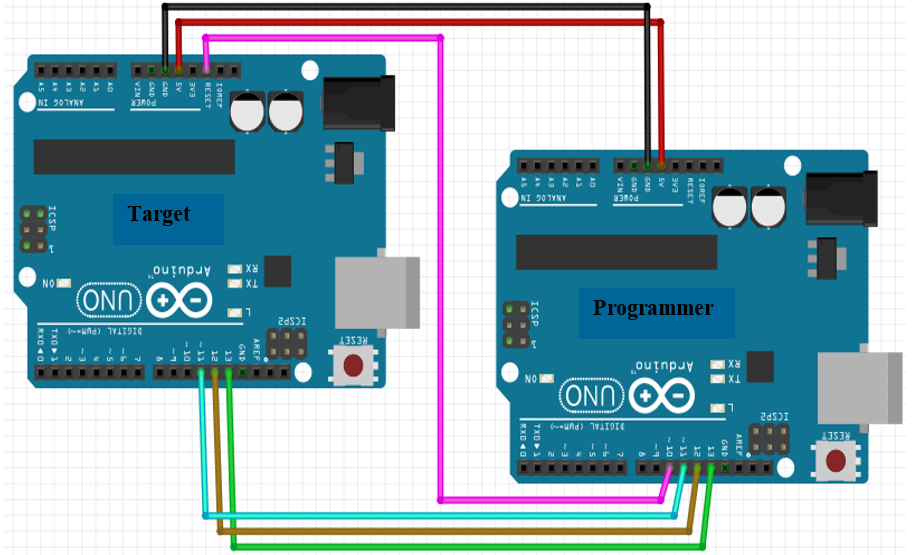
\includegraphics[scale=0.3]{EXP_10_Images/fig1.png}
\end{center}
\begin{center} {Figure 1. Non- Inverting Op-Amp}\end{center}

\noindent In the above circuit, we connect an external resistance R1 and feedback resistance R2 at inverting input. Now, by applying Kirchhoff Current Law, we will get :

\begin{center}  $ V_o_u_t/V_i_n= 1+(R_2/R_1) $  \end{center}


\noindent The closed-loop gain of the circuit is:
\begin{center} $ A= 1+(R_2/R_1) $ \end{center}


\begin{center} 
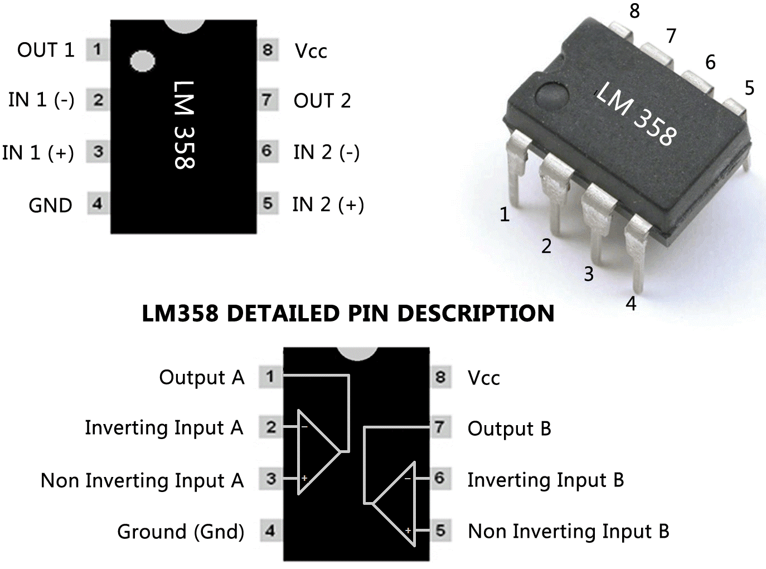
\includegraphics[scale=0.65]{EXP_10_Images/fig2.png}
\end{center}
\begin{center} {Figure 2.LM358 IC Pinout }\\[21pt]\end{center}

\noindent In this experiment, we are going to use an LM358 operational amplifier for making a non-inverting amplifier of gain(A) 10. Follow the circuit diagram as shown below to make a non-inverting op-amp using LM328. Here the external resistance R1 is 1k$\Omega$ and feedback resistance R2 is 10k$\Omega$.\\

\noindent \textbf{\large PROCEDURE}
\begin{enumerate}
\setlength\itemsep{-0.3em}
\item Do the connection as shown in figure 3 and figure 4. 

\item By turning the knob, set the voltage across pin 3 and pin 2 of the potentiometer at 0.3V (approx), measuring through the multimeter. This is the supply ($V_i_n$)  voltage to be amplified.

\item Measure the voltage across GND and Pin 1 of LM358 (i.e. $V_o_u_t$).

\item Note the both $V_i_n$ and $V_o_u_t$.




\vspace{20mm}
\begin{center} 
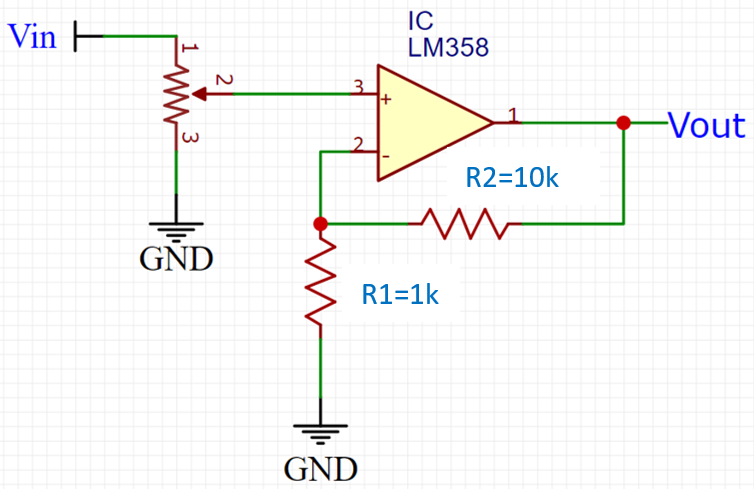
\includegraphics[scale=0.7]{EXP_10_Images/fig3.PNG}
\end{center}
\begin{center} {Figure 3. Circuit Diagram of Non-Inverting Amplifier using LM358}\end{center}

\begin{center} 
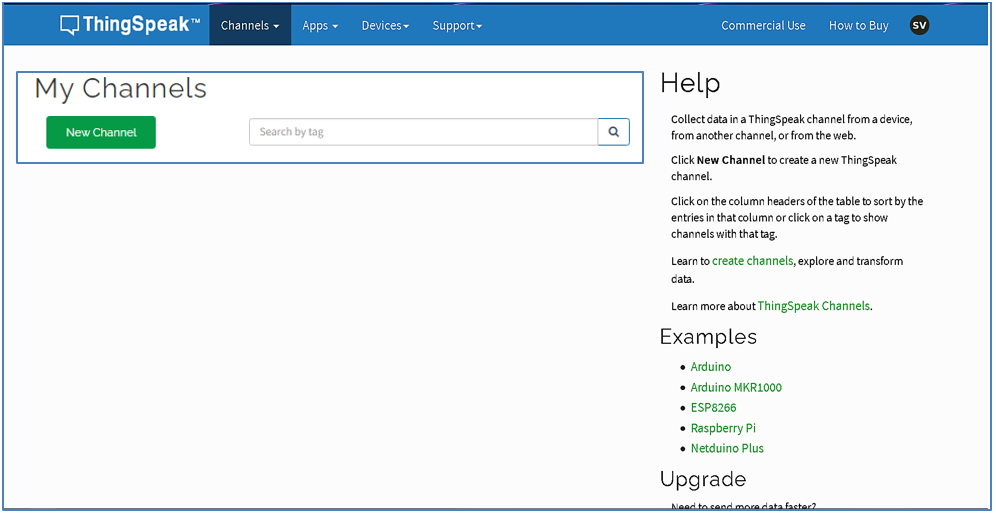
\includegraphics[scale=0.8]{EXP_10_Images/fig4.PNG}
\end{center}
\begin{center} {Figure 4. Circuit realization in Breadboard}\end{center}

\item Repeat the step 3 and 4 by setting Vin (Potentiometer voltage a/c pin 2&3) at 0.4, 0.5, 0.6, and so on. Note the Vin and Vout each time.\\

\noindent \textbf{Expected outcome:} We will observe that the voltage will amplify 11 times (but not greater than input voltage).


\end{enumerate}

\textbf{\large REFERENCES:}
\vspace{-6mm}
\begin{enumerate}
\setlength\itemsep{-0.3em}
\item  \href {http://www.learningaboutelectronics.com/Articles/Non-inverting-op-amp-circuit.php}{How to Build a Non-inverting Op Amp Circuit }
\item  \href {https://www.componentsinfo.com/ic-lm358-pinout-equivalent/}{IC LM358 Pinout, Equivalent, Applications \& Other Info - Components Info}
\end{enumerate}

\end{justify}
\end{document}